\documentclass[12pt,a4paper]{article}
\usepackage{ctex}
\usepackage{amsmath,amscd,amsbsy,amssymb,latexsym,url,bm,amsthm}
\usepackage{epsfig,graphicx,subfigure}
\usepackage{enumitem,balance}
\usepackage{wrapfig}
\usepackage{mathrsfs,euscript}
\usepackage[usenames]{xcolor}
\usepackage{hyperref}
\usepackage[vlined,ruled,linesnumbered]{algorithm2e}
\usepackage{array}
\usepackage{caption}
\hypersetup{colorlinks=true,linkcolor=black}

\newtheorem{theorem}{Theorem}
\newtheorem{lemma}[theorem]{Lemma}
\newtheorem{proposition}[theorem]{Proposition}
\newtheorem{corollary}[theorem]{Corollary}
\newtheorem{exercise}{Exercise}
\newtheorem*{solution}{Solution}
\newtheorem{definition}{Definition}
\theoremstyle{definition}

\renewcommand{\thefootnote}{\fnsymbol{footnote}}

\newcommand{\postscript}[2]
 {\setlength{\epsfxsize}{#2\hsize}
  \centerline{\epsfbox{#1}}}

\renewcommand{\baselinestretch}{1.0}

\setlength{\oddsidemargin}{-0.365in}
\setlength{\evensidemargin}{-0.365in}
\setlength{\topmargin}{-0.3in}
\setlength{\headheight}{0in}
\setlength{\headsep}{0in}
\setlength{\textheight}{10.1in}
\setlength{\textwidth}{7in}
\makeatletter \renewenvironment{proof}[1][Proof] {\par\pushQED{\qed}\normalfont\topsep6\p@\@plus6\p@\relax\trivlist\item[\hskip\labelsep\bfseries#1\@addpunct{.}]\ignorespaces}{\popQED\endtrivlist\@endpefalse} \makeatother
\makeatletter
\renewenvironment{solution}[1][Solution] {\par\pushQED{\qed}\normalfont\topsep6\p@\@plus6\p@\relax\trivlist\item[\hskip\labelsep\bfseries#1\@addpunct{.}]\ignorespaces}{\popQED\endtrivlist\@endpefalse} \makeatother

\begin{document}
\noindent
\captionsetup[figure]{labelfont={bf},labelformat={default},labelsep=period,name={Fig.}}
%========================================================================
\noindent\framebox[\linewidth]{\shortstack[c]{
\Large{\textbf{Lab07-Amortized Analysis}}\vspace{1mm}\\
CS214-Algorithm and Complexity, Xiaofeng Gao, Spring 2020.}}
\begin{center}
\footnotesize{\color{red}$*$ If there is any problem, please contact TA Shuodian Yu. }

\footnotesize{\color{blue}$*$ Name:Haotian Xue  \quad Student ID:518021910506 \quad Email: xavihart@sjtu.edu.cn}
\end{center}
\begin{enumerate}
	\item For the TABLE-DELETE Operation in Dynamic Tables, suppose we construct a table by multiplying its size by $\frac 23$ when the load factor drops below $\frac 13$. Using \emph{Potential Method} to prove that the amortized cost of a TABLE-DELETE that uses this strategy is bounded above by a constant.
	
	\begin{solution}
		The solution for this problem is as follows.

		Since we only need to calculate the amortized cost of TABLE-DELETE operation,  we do not need to take into
		account the expansion of the table.
		
		We can set the potential function as $\Phi_i = s_i - n_i$, where $n_i$ and $s_i$ are the number of elements in the table and the size of table after the $i$th operation respectively.
	$s_0 - n_0 = 0$ and for any $i \in \mathbb{N}$, $\Phi_i \geq 0$.
		
		Then we do the delete operation:
		
		\begin{itemize}
			\item \textbf{Case1}: The contraction is not triggered.
	
			Then we have: $n_i = n_{i-1} - 1$, $s_i = s_{i-1}$, and the amortized cost is:

			\begin{gather*}
				\hat{C}_i = C_i + \Phi_{i} - \Phi_{i-1} \\
				 = 1 + (s_i - n_i) - (s_{i - 1} - n_{i - 1})\\
				 = 1 + (s_i - s_{i - 1}) + (n_{i - 1} - n_{i}) =2
			\end{gather*}

			\item \textbf{Case2}: The contraction is triggered.
			
			Then we have: $n_i = n_{i-1} - 1$, $s_i = \frac{2}{3}s_{i-1}$, $n_i = \frac{1}{3}s_{i-1}$, and the amortized cost is:
			
			\begin{gather*}
				\hat{C}_i = C_i + \Phi_{i} - \Phi_{i-1} \\
				 = n_i + 1 + (s_i - n_i) - (s_{i - 1} - n_{i - 1})\\
				 = n_i + (s_i - s_{i - 1}) + (n_{i - 1} - n_{i}) \\
				 = n_i - \frac{1}{3}s_{i-1} + 1 = 1\\
			\end{gather*}


		\end{itemize}
		  
	Considering the two cases above, we can safely get the amortized cost for DELETE-TABLE operation is $O(1)$.

	\textbf{P.S.} Actually, we can use many other potential functions and their universal form may be $s_i + kn_i$, where $k \in \{x|x\geq -1, x\in \mathbb{Z}\}$.
	That is because $n_i$ always satisfies $n_i = n_{i - 1} - 1$.

		
	\end{solution}



	\item A \textbf{multistack} consists of an infinite series of stacks $S_0, S_1, S_2,\cdots$, where the $i^{th}$ stack $S_i$ can hold up to $3^i$ elements. Whenever a user attempts to push an element onto any full stack $S_i$, we first pop all the elements off $S_i$ and push them onto stack $S_{i+1}$ to make room. (Thus, if $S_{i+1}$ is already full, we first recursively move all its members to $S_{i+2}$ .) An illustrative example is shown in Figure \ref{Fig-MultiStack}. Moving a single element from one stack to the next takes $O(1)$ time. If we push a new element, \underline{we always intend to push it in stack $S_0$}.

	\begin{figure}[!htbp]
	\centering
	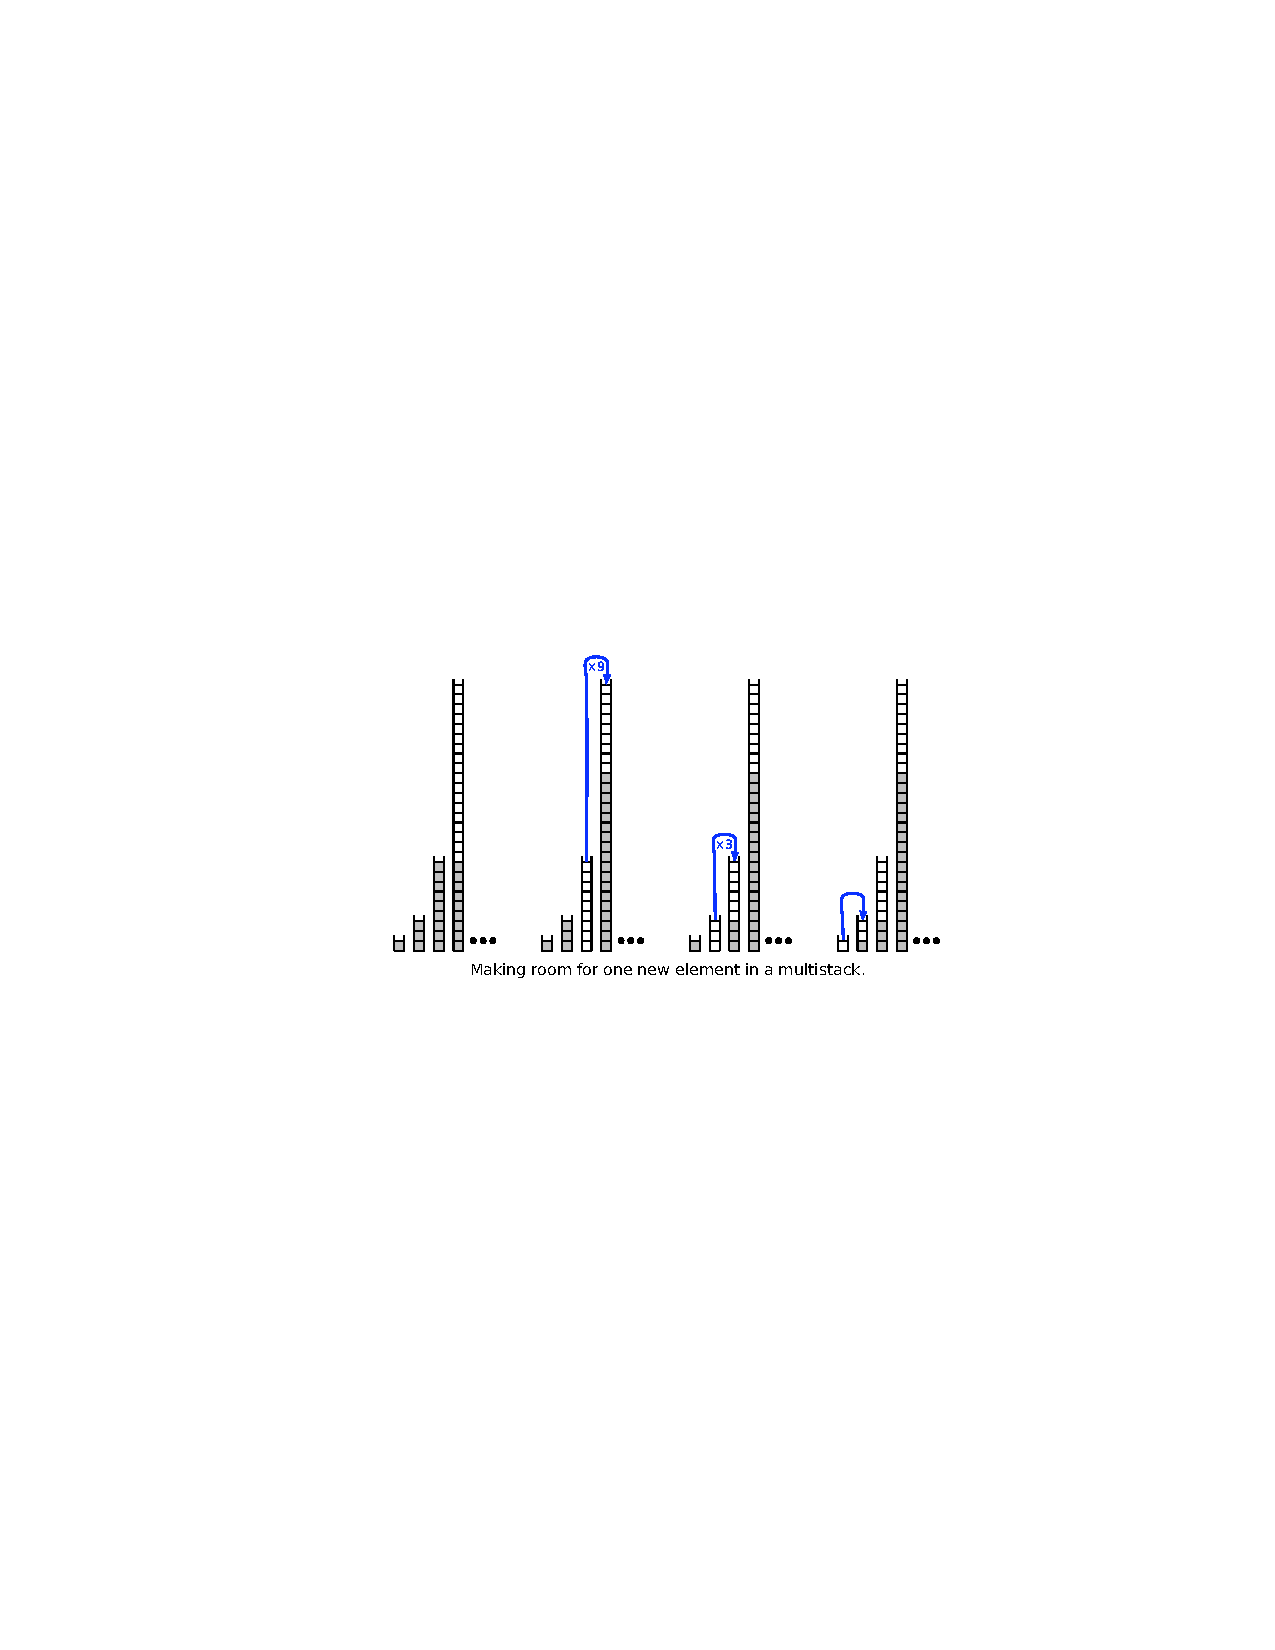
\includegraphics[width=0.5\textwidth]{Fig-MultiStack.pdf}
	\caption{An example of making room for one new element in a multistack.}
	\label{Fig-MultiStack}
	\end{figure}



    \begin{enumerate}
        \item In the worst case, how long does it take to push a new element onto a multistack containing $n$ elements?
        \item Prove that the amortized cost of a push operation is $O(\log n)$ by \emph{Aggregation Analysis}.
        \item {\color{red}(Optional Subquestion with Bonus)} Prove that the amortized cost of a push operation is $O(\log n)$ by \emph{Potential Method}.
	\end{enumerate}
	
   \begin{solution}
	The solution for this problem is as follows.
	
	We first define the \textbf{depth} of an element in a stack : if element $a$ is in $Si$, then the depth of $a$ is $d(a) = i + 1$. Also we note the 
	cost for inserting the $i$th element is $C_i$ and the total cost spent on specific element $a$ to get the current situation is $CT(a)$.

	(a) In the worst case, the $S_0$ to $S_k$ are all full so we need to move every stack to make room for the inserted element, so we have $n = 1+3^2+...+3^i$, the cost for inserting an element now is :
	$C_{n+1} = 1+1+3+3^2+...+3^k = n+1$, $k=O(\log n)$. So the cost is $O(n)$ in worst cases.
   
	 (b) To get the amortized cost for each insert operation, we assume now $S_0$ to $S_i$ is full and we should calculate the total cost $T(n)$ for inserting $n = 1+3+...+3^i$ elements.
	 
	 \begin{equation*}
		 T(n) = \sum_{i=1}^{n}C_i = \sum_{a} CT(a)
	 \end{equation*}

	 The equation above transfer calculating the sum of cost for each step into calculating 
	 the sum of cost for each element, and we actually have:

	 \begin{equation*}
		CT(a) = d(a)
	\end{equation*}

	 So we can get the total cost by tranversing each stacks since elements in the same stack share the same depth:
	
	\begin{equation*}
       T(n) = \sum_{i = 0}^{k} 3^{i} * (i+1) =  O(k3^k) = O(n\log n)
	\end{equation*}
	
	The amortized cost is $C = \frac{T(n)}{n} = O(\log n)$.

	 
   (c) We define $N_{i}^{n}$ as the number of elements in $S_i$ after $n$ push operation. And we define $D(n)$ to be the maximum depth of elements after $n$ push operations.
   Also we make $f(n) = \log (2n+1)$ and it is obvious that:
	   $D(n) < f(n)$.

	   To get the amortized cost, we define the potential function as:

	   \begin{equation*}
		   \Phi_n = \sum_{i=1}^{D(n)}N_{i}^{n}(f(n) - i)
	   \end{equation*}

	   $\Phi_0 = 0$, $\Phi_i(i=1, 2, ..)$ is always positive since $D(n) < f(n)$. 

	   Then we have $\hat{C_n} = C_n + \Phi_n - \Phi_{n - 1}$:

	   \begin{gather*}
		\hat{C_n} = C_n + \sum_{i=1}^{D(n)}N_{i}^{n}(f(n) - i) - \sum_{i=1}^{D(n-1)}N_{i}^{n-1}(f(n-1) - i)\\
				= (f(n)\sum_{i=1}^{D(n)}N_{i}^{n} - f(n-1)\sum_{i=1}^{D(n-1)}N_{i}^{n-1}) + (\sum_{i=1}^{D(n-1)}iN_{i}^{n-1} - \sum_{i=1}^{D(n)}iN_{i}^{n} + C_n)\\
				= (nf(n) - (n-1)f(n-1)) + C_n + P_n = O(\log n) + (P_n + C_n) \\
	   \end{gather*}

	   We can see $C_n + P_n$ from the angle of elements, we want to calculate the \textbf{effect of one element $a$} and then tranverse all of the elements, that is:
	  
	   \begin{equation*}
		C_n + P_n = \sum_{a}c_a - \sum_{a}\Delta{N_a} = \sum_{a}(c_a - \Delta{N_a})
	   \end{equation*}

	   where $\Delta{N_a}$ is the effect $a$ has caused to the change of $P_n$. Then there are two cases for states of $a$:

	   \begin{itemize}
		   \item \textbf{Case 1:} $a$ is not moved from one stack to another.
		   
		   Then we have $c_a - \Delta{N_a} = 0 - 0 =0$.

		   \item \textbf{Case 1:} $a$ is not moved from one stack to another.
		   
		   Suppose we move $a$ from $S_i$ to $S_{i+1}$
		   ,then we have $c_a - \Delta{N_a} = 1 - (i\times(0-1) + (i+1)\times(1-0)) = 0$. 
		\end{itemize}

		So finally we have: $\hat{C_n} = O(\log n)$. Which in fact prove the amortized cost to be $O(\log n)$.

	

   



\end{solution}

	\item Given a graph $G = (V, E)$, and let $V'$ be a strict subset of $V$. Prove the following propositions.
	
	\begin{enumerate}
		\item Let $T$ be a minimum spanning tree of a $G$. Let $T'$ be the subgraph of $T$ induced by $V'$, and let $G'$ be the subgraph of $G$ induced by $V'$. Then $T'$ is a minimum spanning tree of $G'$ if $T'$ is connected.
		\item Let $e$ be a minimum weight edge which connects $V'$ and $V \setminus V'$. There exists a minimum weight spanning tree which contains e.
	\end{enumerate}



\begin{solution}
	We can prove these two problems by contradction.

(a) If $T^{'}$ is not the MST of $G^{'}$, then there must exists one subtree $T^{''}$ of $T$ which is the 
MST of $G^{'}$ and the sum of weights of $T^{''}$ is less than that of $T^{'}$. We think about $T_0 = (T\setminus T^{'})\cup T^{''}$ which is a spanning tree 
 for $G$. However the total weights of $T_0$ is less than that of $T$, which contradicts the fact that $T$ is the MST of $G$.

(b) If there is no MST that contains $e$, then we just pick one MST $T$ which satisfies $e \notin T$. Then we add $e$ to $T$ to get $T_0 = \{e\} \cup T$. 
It is obvious that it will generate a cycle $C \subset T_0$ and $e \in C$. If all vertex of edges in $C - \{e\}$ is in either $V^{'}$ or $V \setminus V^{'}$, then we note $u\in V^{'},v \in V \setminus V^{'}$
are the two vertexes of $e$, if we start from $u$ then we can only get to vertexes in $V$, such that we cannot get to $v$. So there must exists another edge $e_0$ in 
the cycle which connects $V^{'}$ and $V\setminus V^{'}$. If we replace $e_0$ with $e$ in $T$ to get $T^{'} = T \setminus \{e_0\} \cup \{e\} $, then $T^{'}$ is 
obviously a spanning tree and its weight is less than that of $T$, which is contradictory with the fact that $T$ is a MST.

\begin{figure}[!htbp]
	\centering
	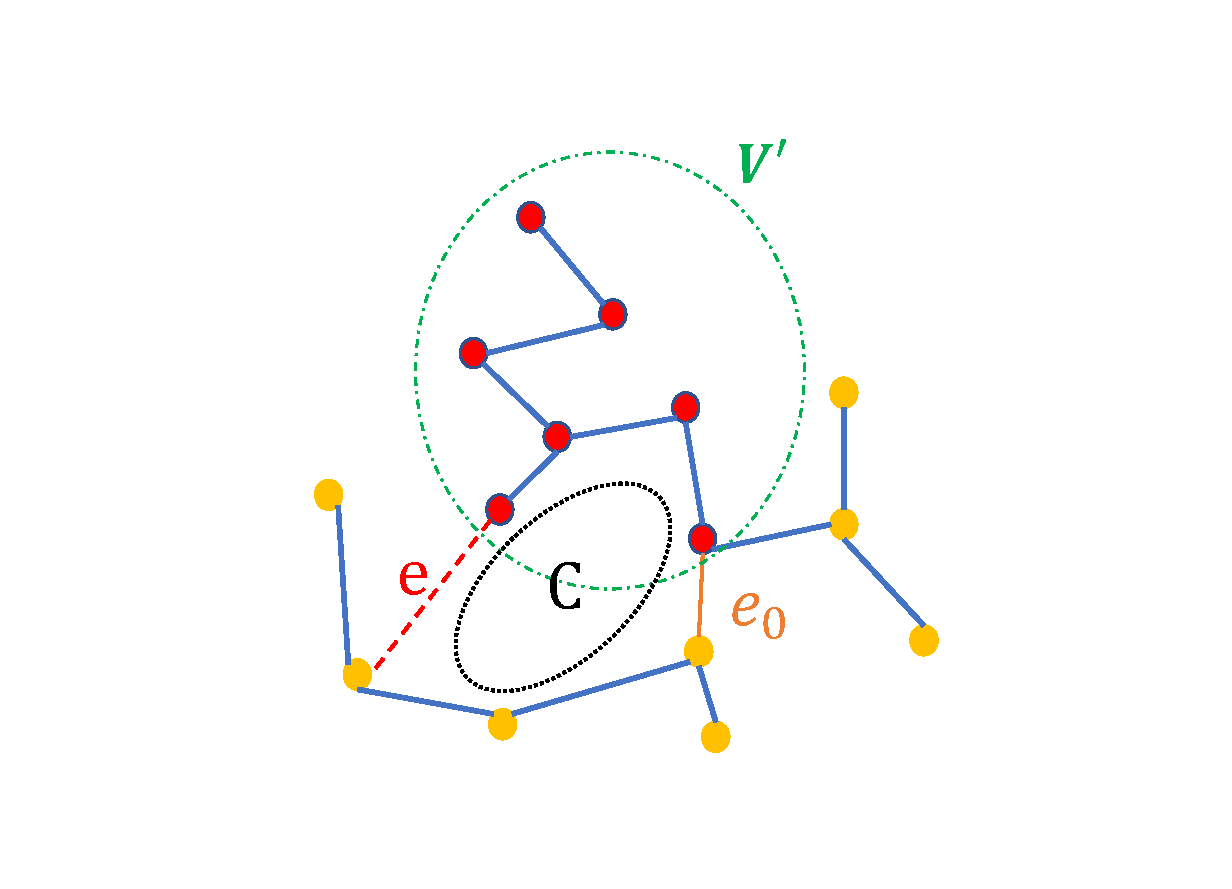
\includegraphics[width=0.6\textwidth]{32.pdf}
	\caption{An illustration for (b) in Problem3.}
	\label{Fig-MultiStack}
	\end{figure}


\end{solution}

\end{enumerate}

\textbf{Remark:} Please include your .pdf, .tex files for uploading with standard file names.


%========================================================================
\end{document}
